% Created by tikzDevice version 0.7.0 on 2014-08-02 12:37:24
% !TEX encoding = UTF-8 Unicode
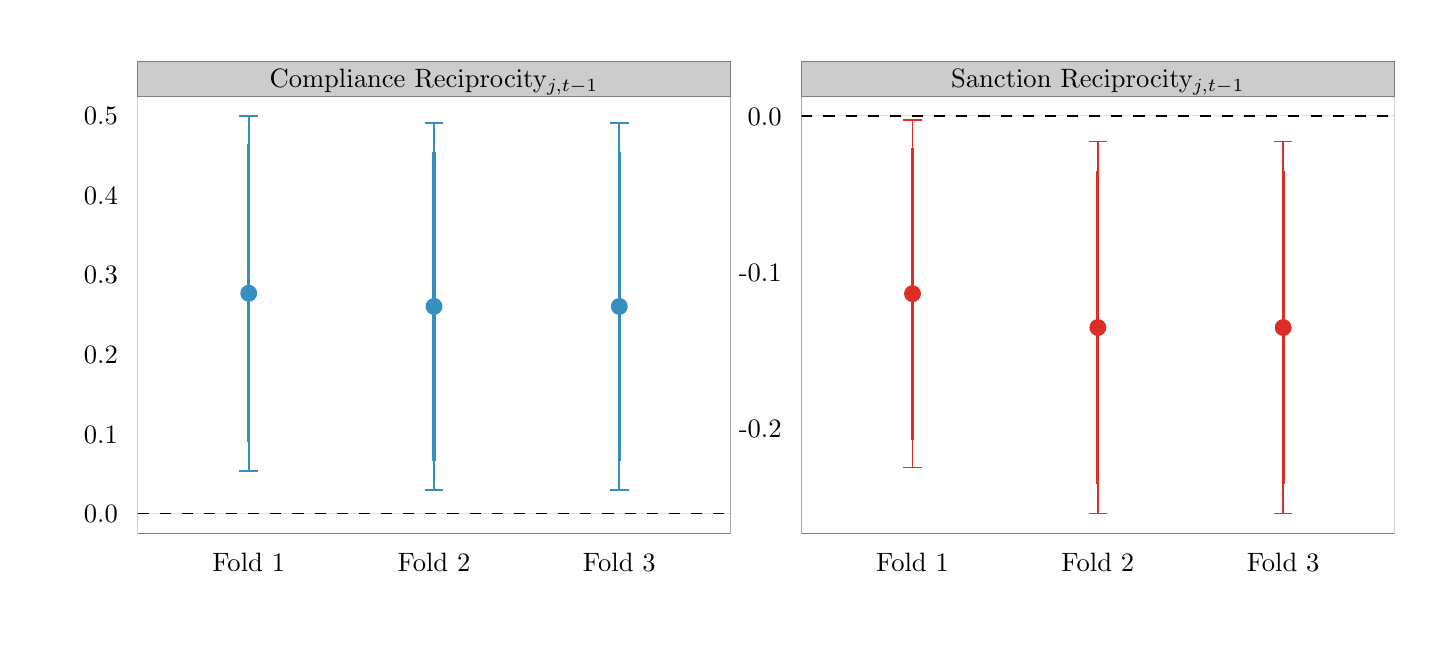
\begin{tikzpicture}[x=1pt,y=1pt]
\definecolor[named]{fillColor}{rgb}{1.00,1.00,1.00}
\path[use as bounding box,fill=fillColor,fill opacity=0.00] (0,0) rectangle (505.89,216.81);
\begin{scope}
\path[clip] (  0.00,  0.00) rectangle (505.89,216.81);
\definecolor[named]{drawColor}{rgb}{1.00,1.00,1.00}
\definecolor[named]{fillColor}{rgb}{1.00,1.00,1.00}

\path[draw=drawColor,line width= 0.6pt,line join=round,line cap=round,fill=fillColor] (  0.00,  0.00) rectangle (505.89,216.81);
\end{scope}
\begin{scope}
\path[clip] ( 39.69, 34.03) rectangle (253.97,192.13);
\definecolor[named]{fillColor}{rgb}{1.00,1.00,1.00}

\path[fill=fillColor] ( 39.69, 34.03) rectangle (253.97,192.13);
\definecolor[named]{drawColor}{rgb}{0.21,0.56,0.75}
\definecolor[named]{fillColor}{rgb}{0.21,0.56,0.75}

\path[draw=drawColor,draw opacity=0.30,line width= 0.3pt,line join=round,fill=fillColor,fill opacity=0.30] ( 79.87, 56.72) -- ( 79.87,184.94);

\path[draw=drawColor,draw opacity=0.30,line width= 0.3pt,line join=round,fill=fillColor,fill opacity=0.30] (146.83, 49.71) -- (146.83,182.42);

\path[draw=drawColor,draw opacity=0.30,line width= 0.3pt,line join=round,fill=fillColor,fill opacity=0.30] (213.79, 49.71) -- (213.79,182.42);
\definecolor[named]{drawColor}{rgb}{0.21,0.56,0.75}
\definecolor[named]{fillColor}{rgb}{0.21,0.56,0.75}

\path[draw=drawColor,line width= 1.1pt,line join=round,fill=fillColor] ( 79.87, 67.03) -- ( 79.87,174.64);

\path[draw=drawColor,line width= 1.1pt,line join=round,fill=fillColor] (146.83, 60.38) -- (146.83,171.75);

\path[draw=drawColor,line width= 1.1pt,line join=round,fill=fillColor] (213.79, 60.38) -- (213.79,171.75);
\definecolor[named]{drawColor}{rgb}{0.00,0.00,0.00}
\definecolor[named]{fillColor}{rgb}{0.00,0.00,0.00}

\path[draw=drawColor,line width= 0.6pt,dash pattern=on 4pt off 4pt ,line join=round,fill=fillColor] ( 39.69, 41.22) -- (253.97, 41.22);
\definecolor[named]{drawColor}{rgb}{0.21,0.56,0.75}
\definecolor[named]{fillColor}{rgb}{0.21,0.56,0.75}

\path[draw=drawColor,line width= 0.4pt,line join=round,line cap=round,fill=fillColor] ( 79.87,120.83) circle (  2.85);

\path[draw=drawColor,line width= 0.4pt,line join=round,line cap=round,fill=fillColor] (146.83,116.07) circle (  2.85);

\path[draw=drawColor,line width= 0.4pt,line join=round,line cap=round,fill=fillColor] (213.79,116.07) circle (  2.85);

\path[draw=drawColor,line width= 0.6pt,line join=round] ( 76.52,184.94) --
	( 83.21,184.94);

\path[draw=drawColor,line width= 0.6pt,line join=round] ( 79.87,184.94) --
	( 79.87, 56.72);

\path[draw=drawColor,line width= 0.6pt,line join=round] ( 76.52, 56.72) --
	( 83.21, 56.72);

\path[draw=drawColor,line width= 0.6pt,line join=round] (143.48,182.42) --
	(150.18,182.42);

\path[draw=drawColor,line width= 0.6pt,line join=round] (146.83,182.42) --
	(146.83, 49.71);

\path[draw=drawColor,line width= 0.6pt,line join=round] (143.48, 49.71) --
	(150.18, 49.71);

\path[draw=drawColor,line width= 0.6pt,line join=round] (210.45,182.42) --
	(217.14,182.42);

\path[draw=drawColor,line width= 0.6pt,line join=round] (213.79,182.42) --
	(213.79, 49.71);

\path[draw=drawColor,line width= 0.6pt,line join=round] (210.45, 49.71) --
	(217.14, 49.71);
\definecolor[named]{drawColor}{rgb}{0.50,0.50,0.50}

\path[draw=drawColor,line width= 0.6pt,line join=round,line cap=round] ( 39.69, 34.03) rectangle (253.97,192.13);
\end{scope}
\begin{scope}
\path[clip] (279.56, 34.03) rectangle (493.85,192.13);
\definecolor[named]{fillColor}{rgb}{1.00,1.00,1.00}

\path[fill=fillColor] (279.56, 34.03) rectangle (493.85,192.13);
\definecolor[named]{drawColor}{rgb}{0.87,0.18,0.15}
\definecolor[named]{fillColor}{rgb}{0.87,0.18,0.15}

\path[draw=drawColor,draw opacity=0.30,line width= 0.3pt,line join=round,fill=fillColor,fill opacity=0.30] (319.74, 57.83) -- (319.74,183.54);

\path[draw=drawColor,draw opacity=0.30,line width= 0.3pt,line join=round,fill=fillColor,fill opacity=0.30] (386.70, 41.22) -- (386.70,175.67);

\path[draw=drawColor,draw opacity=0.30,line width= 0.3pt,line join=round,fill=fillColor,fill opacity=0.30] (453.67, 41.22) -- (453.67,175.67);
\definecolor[named]{drawColor}{rgb}{0.87,0.18,0.15}
\definecolor[named]{fillColor}{rgb}{0.87,0.18,0.15}

\path[draw=drawColor,line width= 1.1pt,line join=round,fill=fillColor] (319.74, 67.94) -- (319.74,173.43);

\path[draw=drawColor,line width= 1.1pt,line join=round,fill=fillColor] (386.70, 52.03) -- (386.70,164.86);

\path[draw=drawColor,line width= 1.1pt,line join=round,fill=fillColor] (453.67, 52.03) -- (453.67,164.86);
\definecolor[named]{drawColor}{rgb}{0.00,0.00,0.00}
\definecolor[named]{fillColor}{rgb}{0.00,0.00,0.00}

\path[draw=drawColor,line width= 0.6pt,dash pattern=on 4pt off 4pt ,line join=round,fill=fillColor] (279.56,184.94) -- (493.85,184.94);
\definecolor[named]{drawColor}{rgb}{0.87,0.18,0.15}
\definecolor[named]{fillColor}{rgb}{0.87,0.18,0.15}

\path[draw=drawColor,line width= 0.4pt,line join=round,line cap=round,fill=fillColor] (319.74,120.69) circle (  2.85);

\path[draw=drawColor,line width= 0.4pt,line join=round,line cap=round,fill=fillColor] (386.70,108.45) circle (  2.85);

\path[draw=drawColor,line width= 0.4pt,line join=round,line cap=round,fill=fillColor] (453.67,108.45) circle (  2.85);

\path[draw=drawColor,line width= 0.6pt,line join=round] (316.39,183.54) --
	(323.09,183.54);

\path[draw=drawColor,line width= 0.6pt,line join=round] (319.74,183.54) --
	(319.74, 57.83);

\path[draw=drawColor,line width= 0.6pt,line join=round] (316.39, 57.83) --
	(323.09, 57.83);

\path[draw=drawColor,line width= 0.6pt,line join=round] (383.35,175.67) --
	(390.05,175.67);

\path[draw=drawColor,line width= 0.6pt,line join=round] (386.70,175.67) --
	(386.70, 41.22);

\path[draw=drawColor,line width= 0.6pt,line join=round] (383.35, 41.22) --
	(390.05, 41.22);

\path[draw=drawColor,line width= 0.6pt,line join=round] (450.32,175.67) --
	(457.01,175.67);

\path[draw=drawColor,line width= 0.6pt,line join=round] (453.67,175.67) --
	(453.67, 41.22);

\path[draw=drawColor,line width= 0.6pt,line join=round] (450.32, 41.22) --
	(457.01, 41.22);
\definecolor[named]{drawColor}{rgb}{0.50,0.50,0.50}

\path[draw=drawColor,line width= 0.6pt,line join=round,line cap=round] (279.56, 34.03) rectangle (493.85,192.13);
\end{scope}
\begin{scope}
\path[clip] (  0.00,  0.00) rectangle (505.89,216.81);
\definecolor[named]{drawColor}{rgb}{0.50,0.50,0.50}
\definecolor[named]{fillColor}{rgb}{0.80,0.80,0.80}

\path[draw=drawColor,line width= 0.2pt,line join=round,line cap=round,fill=fillColor] ( 39.69,192.13) rectangle (253.97,204.77);
\definecolor[named]{drawColor}{rgb}{0.00,0.00,0.00}

\node[text=drawColor,anchor=base,inner sep=0pt, outer sep=0pt, scale=  0.96] at (146.83,195.14) {Compliance Reciprocity$_{j,t-1}$};
\end{scope}
\begin{scope}
\path[clip] (  0.00,  0.00) rectangle (505.89,216.81);
\definecolor[named]{drawColor}{rgb}{0.50,0.50,0.50}
\definecolor[named]{fillColor}{rgb}{0.80,0.80,0.80}

\path[draw=drawColor,line width= 0.2pt,line join=round,line cap=round,fill=fillColor] (279.56,192.13) rectangle (493.85,204.77);
\definecolor[named]{drawColor}{rgb}{0.00,0.00,0.00}

\node[text=drawColor,anchor=base,inner sep=0pt, outer sep=0pt, scale=  0.96] at (386.70,195.14) {Sanction Reciprocity$_{j,t-1}$};
\end{scope}
\begin{scope}
\path[clip] (  0.00,  0.00) rectangle (505.89,216.81);
\definecolor[named]{drawColor}{rgb}{0.00,0.00,0.00}

\node[text=drawColor,anchor=base east,inner sep=0pt, outer sep=0pt, scale=  0.96] at ( 32.57, 37.91) {0.0};

\node[text=drawColor,anchor=base east,inner sep=0pt, outer sep=0pt, scale=  0.96] at ( 32.57, 66.70) {0.1};

\node[text=drawColor,anchor=base east,inner sep=0pt, outer sep=0pt, scale=  0.96] at ( 32.57, 95.49) {0.2};

\node[text=drawColor,anchor=base east,inner sep=0pt, outer sep=0pt, scale=  0.96] at ( 32.57,124.28) {0.3};

\node[text=drawColor,anchor=base east,inner sep=0pt, outer sep=0pt, scale=  0.96] at ( 32.57,153.06) {0.4};

\node[text=drawColor,anchor=base east,inner sep=0pt, outer sep=0pt, scale=  0.96] at ( 32.57,181.85) {0.5};
\end{scope}
\begin{scope}
\path[clip] (  0.00,  0.00) rectangle (505.89,216.81);
\definecolor[named]{drawColor}{rgb}{0.00,0.00,0.00}

\node[text=drawColor,anchor=base east,inner sep=0pt, outer sep=0pt, scale=  0.96] at (272.45, 68.69) {-0.2};

\node[text=drawColor,anchor=base east,inner sep=0pt, outer sep=0pt, scale=  0.96] at (272.45,125.17) {-0.1};

\node[text=drawColor,anchor=base east,inner sep=0pt, outer sep=0pt, scale=  0.96] at (272.45,181.64) {0.0};
\end{scope}
\begin{scope}
\path[clip] (  0.00,  0.00) rectangle (505.89,216.81);
\definecolor[named]{drawColor}{rgb}{0.00,0.00,0.00}

\node[text=drawColor,anchor=base,inner sep=0pt, outer sep=0pt, scale=  0.96] at ( 79.87, 20.31) {Fold 1};

\node[text=drawColor,anchor=base,inner sep=0pt, outer sep=0pt, scale=  0.96] at (146.83, 20.31) {Fold 2};

\node[text=drawColor,anchor=base,inner sep=0pt, outer sep=0pt, scale=  0.96] at (213.79, 20.31) {Fold 3};
\end{scope}
\begin{scope}
\path[clip] (  0.00,  0.00) rectangle (505.89,216.81);
\definecolor[named]{drawColor}{rgb}{0.00,0.00,0.00}

\node[text=drawColor,anchor=base,inner sep=0pt, outer sep=0pt, scale=  0.96] at (319.74, 20.31) {Fold 1};

\node[text=drawColor,anchor=base,inner sep=0pt, outer sep=0pt, scale=  0.96] at (386.70, 20.31) {Fold 2};

\node[text=drawColor,anchor=base,inner sep=0pt, outer sep=0pt, scale=  0.96] at (453.67, 20.31) {Fold 3};
\end{scope}
\end{tikzpicture}
